\chapter{Technique Overview}\label{ch:research}
This part of the thesis constitutes the main part.
The objective is to create an overview of techniques in the field which may be used to solve the
problem detailed in Chapter~\ref{ch:problem}.
First the search for literature which lays the foundation for the subsequent sections, is documented.
The a taxonomy is introduced which facilitates the analysis and comparison of techniques.
Lastly, the advances in the field are placed in the correct position and analyzed.

\section{Literature Search}\label{se:litSearch}
This section documents the search for literature which provides the content for the subsequent
overview.
For this, important pipelines and notable advances along with their properties are researched,
analysed and presented.
The literature is identified through searching in the Google Scholar database.
The search is executed with keywords such as, but not only: Deep Learning, Text Detection,
Text Recognition, Text Spotting, Scene Text, Pipeline.
% FIXME: update keywords
A criterion for further examination is an appropriate amount of citations for the piece of literature
in question.
Additionally, literature is selected through citations for and by literature which has already been
identified as important.
All research after 2018 which pertains to extracting scene text is regarded as relevant.
Standard \ac{OCR} solutions may not hold validity in practice, as the image and text conditions can
vary in the defined problem~\citep{chen_text_2021}.
The delimination from Section~\ref{se:problem} of course holds for this chapter and only literature
which concerns advances for the \ac{DL} model architecture will be regarded as important for the
scope of this thesis.
This extends to the whole pipeline from preprocessing an image to the final result of the model.

% FIXME: hierarchical graphic with found papers
% FIXME: describe proceeding

\section{Taxonomy of Pipeline Steps}
In order to create the overview the necessary steps in the process of \ac{STS} need to be highlighted,
from preprocessing to classifying the identified text~\citep{long_scene_2021, sourvanos_challenges_2018}.
The ways in which the respective issues for the steps are solved are identified from literature,
listed and explained alongside.

\begin{figure}[ht]
    \centering
    \resizebox{\linewidth}{!}{
\begin{tikzpicture}[
    every node/.style={draw=black,thin,anchor=west, minimum height=2.5em},
    lroot/.style={%
        edge from parent fork down,
        level distance=0.5cm,
        text centered, text width=3cm},
    lone/.style={%
        text centered, text width=3cm,
        level distance=0.5cm},
    ltwo/.style={%
        text centered, text width=3cm,
        level distance=0.5cm},
    lthree/.style={%
        rounded corners,
        grow=down, xshift=-0.8cm,
        text centered, text width=3cm,
        edge from parent path={(\tikzparentnode.205) |- (\tikzchildnode.west)}},
    level1/.style ={level distance=1.2cm},
    level2/.style ={level distance=2.4cm},
    level3/.style ={level distance=3.6cm},
    level4/.style ={level distance=4.8cm},
    level5/.style ={level distance=6.0cm},
    level 1/.style={sibling distance=8cm},
    level 1/.append style={level distance=1.5cm},
    level 2/.style={sibling distance=4cm},
    level 2/.append style={level distance=1.5cm},
]
%   \draw[help lines] (0,0) grid (4,3);

    % lroot
    \node[anchor=south,lroot]{STS}
    [edge from parent fork down]
        child{node [lone] {STD}
            child{node [ltwo] {Regressor \\ based}
                child[lthree,level1] {node {Feature \\ Extraction}}
                child[lthree,level2] {node {BB \\ Regresseion}}
                child[lthree,level3] {node {IOU \\ matching}}
            }
            child{node [ltwo] {Segmentation \\ based}
                child[lthree,level1] {node {Sub-components \\ segmentation}}
                child[lthree,level2] {node {Text \\ reconstruction}}
            }
        }
        %
        child{node [lone] {STR}
            child{node [ltwo] {Regressor \\ based}
                child[lthree,level1] {node {Image \\ preprocessing}}
                child[lthree,level2] {node {Character \\ segmentation}}
                child[lthree,level3] {node {Character \\ recognition}}
            }
            child{node [ltwo] {Segmentation \\ based}
                child[lthree,level1] {node {Image \\ preprocessing}}
                child[lthree,level2] {node {Feature \\ extraction}}
                child[lthree,level3] {node {Sequence \\ modelling}}
                child[lthree,level4] {node {Prediction}}
            }
        }
        %
        child{node [lone] {E2E}
            child{node [ltwo] {Two Stage}
                child[lthree,level1] {node {STD}}
                child[lthree,level2] {node {STR with \\ feature maps}}
            }
            child{node [ltwo] {One Stage}
                child[lthree,level1] {node {STD \& STR \\ Parallel}}
            }
        };

\end{tikzpicture}
}%


\begin{comment}
\begin{tikzpicture}[
    font=\scriptsize,
    edge from parent fork down,
    level distance=1.75cm,
    every node/.style={
            rectangle,
            minimum height=6mm,
            align=center,
            text depth = 0pt,
    },
    edge from parent/.style={draw=black},
    category/.style={Rectangle},
    step/.style={Circle}
]
    \Tree [.STS
        [.{STD}
            [.{Feature \\ Extraction} ]
            [.{BB Regression} ]
        ]
        [.{STR}
            [.{Preprocessing} ]
            [.{Feature \\ Extraction} ]
            [.{Sequence \\ Modelling} ]
            [.{Prediction} ]
        ]
    ]
\end{tikzpicture}
\end{comment}

\caption{Pipeline taxonomy and respective steps\label{fig:pipelineSteps}}
\end{figure}

STD
\begin{itemize}
    \item Two approaches: regression based --- segmentation based (on the rise)
    \item Steps:
        \begin{itemize}
            \item regression based: feature extraction, bounding box regression, IOU matching
            \item segmentation based: segment text areas (different granularity: pixel, component,
                character), assemble text instances (reconstruction)
        \end{itemize}
\end{itemize}

STR
\begin{itemize}
    \item segmentation-free approach (segmentation-based implicit and explicit out of date)
    \item Steps: Preprocessing, Feature Extraction, Sequence Modelling, Prediction
    \item preprocessing, text enhancement: remove distortions, background; improve resolution,
        recover degraded text
        \begin{itemize}
            \item Spatial Transformer Networks (for distortions)
        \end{itemize}
    \item feature extraction: encode image into feature space
        \begin{itemize}
            \item ResNet
                \begin{itemize}
                    \item aggressive downsampling
                    \item $3\times3$ best kernel size
                    \item Gradient saving $\rightarrow$ Res block, Res Bottleneck, Res Grouped
                    \item batch normalization
                    \item 32,50,150,\ldots
                \end{itemize}
            \item GoogLeNet
        \end{itemize}
    \item Sequence and Prediction
        \begin{itemize}
            \item CTC
            \item Encode-Decoder/Attention
            \item Lexicon Free Models!
        \end{itemize}
\end{itemize}

STS
\begin{itemize}
    \item Bestandteile nicht zwangsweise sequentiell
    \item two step or two stage pipeline
\end{itemize}

\begin{comment}
What is segmentation
- Detection: from pixel to character -> better for arbitrary shapes
    - Segmentation
    - Text detection of of segmentation
- Recognition: are not used often (poor word-level results)
    - Segmentation
    - recognition
- End to end?
\end{comment}

\begin{figure}[h]
    \centering
    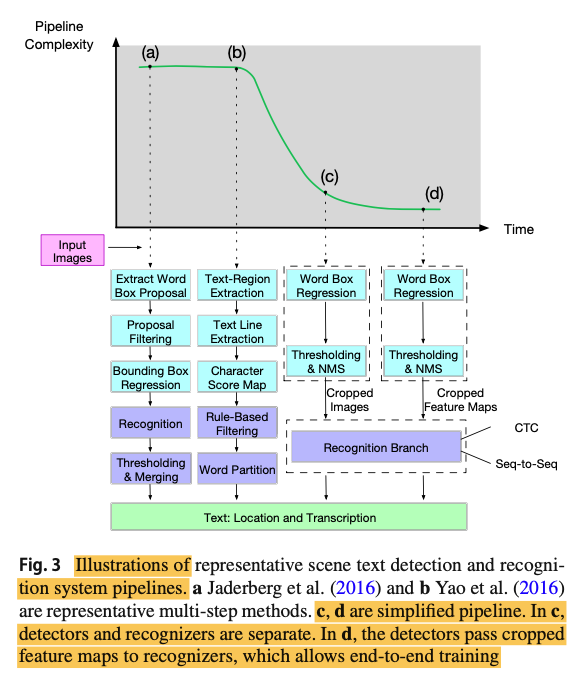
\includegraphics[width=0.60\textwidth]{img/Long-Scene-2021-Pipeline-Changes.png}
    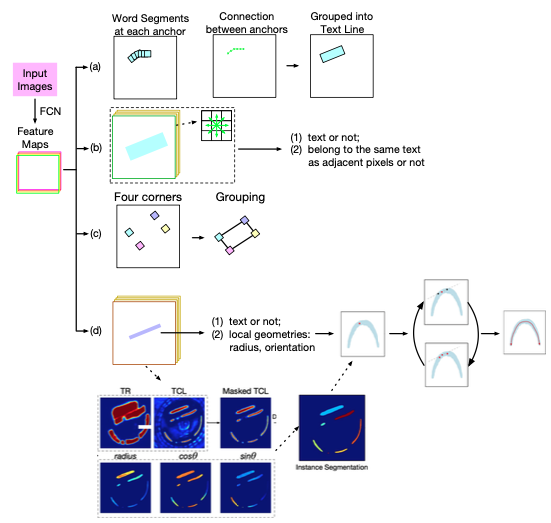
\includegraphics[width=0.60\textwidth]{img/Long-Scene-2021-STD-Pipelines.png}
    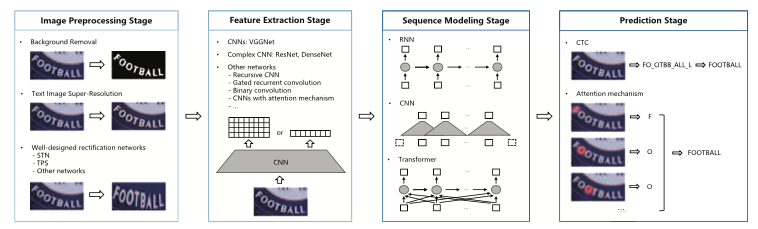
\includegraphics[width=0.60\textwidth]{img/Chen-Text-2021-STR-Pipeline.png}
    \caption{Pipelines~\citep{long_scene_2021,chen_text_2021}\label{fig:piplineChanges}}
\end{figure}

\begin{figure}[ht]
    \centering
    \subfigure[Residual block~\citep{he_deep_2015}\label{fig:residual-block}]{%
        {\scriptsize%
\begin{tikzpicture}[scale=0.6]
    \node (l1) {conv 1};
    \node[right=4mm of l1, label={below:}] (act1) {$\relu$};
    \node[right=4mm of act1] (l2) {conv 2};
    \node[right=4mm of l2,font=\small,label={below:},inner sep=0,pin={60:$F(\X) + \X$}] (add) {$\oplus$};
    \node[right=4mm of add, label={below:}] (act2) {$\relu$};

    \draw[->] (l1) -- (act1);
    \draw[->] (act1) -- (l2);
    \draw[<-] (l1) -- ++(-2,0) node[below, pos=0.8] {$\X$};
    \draw[->] (l2) -- (act2) node[above, pos=0.8] {};
    \draw[->] ($(l1)-(1.5,0)$) to[out=30, in=150] node[below=1ex, midway, align=center]
        {} node[above, midway] {identity} (add);
    \draw[decorate, decoration={brace, amplitude=1ex, raise=1cm}] (l2.east) -- node[midway, below=1.2cm]
        {$F(\X)$} (l1.west);
\end{tikzpicture}
}
%
    }
    \subfigure[Residual block with pooling~\citep{ponti_everything_2017}\label{fig:residual-block}]{%
        {\scriptsize%
\begin{tikzpicture}[scale=0.6]
    \node (l1) {conv 1};
    \node[right=4mm of l1] (l15) {pooling};
    \node[right=4mm of l15, label={below:}] (act1) {$ReLU$};
    \node[right=4mm of act1] (l2) {conv 2};
    \node[right=4mm of l2,font=\Large,label={below:},inner sep=0,pin={90:$F(\X) + P(\X)$}] (add)
        {$\oplus$};
    \node[right=4mm of add, label={below:}] (act2) {$ReLU$};

    \draw[->] (l1) -- (l15);
    \draw[->] (l15) -- (act1);
    \draw[->] (act1) -- (l2);
    \draw[<-] (l1) -- ++(-2,0) node[below, pos=0.8] {$\X$};
    \draw[->] (l2) -- (act2) node[above, pos=0.8] {};
    \draw[->,dashed] ($(l1)-(1.5,0)$) to[out=30, in=150] node[below=1ex, midway, align=center]
        {$P(\X)$} node[above, midway] {pooling} (add);
    \draw[decorate, decoration={brace, amplitude=1ex, raise=1cm}] (l2.east) -- node[midway, below=1.2cm]
        {$F(\X)$} (l1.west);
\end{tikzpicture}
}
%
    }
    \subfigure[Residual bottleneck block~\citep{he_deep_2015}\label{fig:residual-block}]{%
        {\scriptsize%
\begin{tikzpicture}[scale=0.6]
    \node (l1) {conv 1, $1\times1$};
    \node[right=2mm of l1, label={below:}] (act1) {$ReLU$};
    \node[right=2mm of act1] (l15) {conv 2, $3\times3$};
    \node[right=2mm of l15, label={below:}] (act15) {$ReLU$};
    \node[right=2mm of act15] (l2) {conv 3, $1\times1$};
    \node[right=2mm of l2,font=\small,label={below:},inner sep=0,pin={60:$F(\X) + \X$}] (add) {$\oplus$};
    \node[right=2mm of add, label={below:}] (act2) {$ReLU$};

    \draw[->] (l1) -- (act1);
    \draw[->] (act1) -- (l15);
    \draw[->] (l15) -- (act15);
    \draw[->] (act15) -- (l2);
    \draw[<-] (l1) -- ++(-3,0) node[below, pos=0.8] {$\X$};
    \draw[->] (l2) -- (act2) node[above, pos=0.8] {};
    \draw[->] ($(l1)-(2.5,0)$) to[out=30, in=150] node[below=1ex, midway, align=center]
        {} node[above, midway] {identity} (add);
    \draw[decorate, decoration={brace, amplitude=1ex, raise=1cm}] (l2.east) -- node[midway, below=1.2cm]
        {$F(\X)$} (l1.west);
\end{tikzpicture}
}
%
    }
    \caption{Modules introduced with ResNet\label{fig:resnet}}
\end{figure}

\section{State of the Art Methods}

text enhancement:~\cite{chen_text_2021}
model pruning:~\cite{niu_26ms_2019}
integer inference:~\cite{ignatov_ai_2019}
